\documentclass[11pt]{article}

\usepackage{graphicx}
\usepackage[margin=1in]{geometry}
\usepackage[dvipsnames]{xcolor}
\usepackage[most]{tcolorbox}
\usepackage[colorlinks=true, linkcolor=blue]{hyperref}
\usepackage{subcaption,booktabs,float}

\newtcolorbox{definition}[1][]{
  colback=blue!5!white,
  colframe=blue!75!black,
  fonttitle=\bfseries,
  title=Definition: #1
}

\newtcolorbox{warning}[1][]{
  colback=red!5!white,
  colframe=red!75!black,
  fonttitle=\bfseries,
  title=#1
}

\newtcolorbox{note}[1][]{
  colback=green!5!white,
  colframe=green!75!black,
  fonttitle=\bfseries,
  title=#1,
  breakable
}

\newtcolorbox{note_special}[1][]{
  colback=orange!5!white,
  colframe=orange!75!black,
  fonttitle=\bfseries,
  title=#1,
  breakable
}

\begin{document}


\begin{titlepage}
    \centering
    
    
\includegraphics[width=0.4\textwidth]{UCT-logo.png}\\[2cm] 
    
    \textsc{\LARGE University of Cape Town}\\[1.5cm]
    
    \rule{\linewidth}{0.5mm} \\[0.4cm]
    { \huge \bfseries CSC200SS: Computer Science \\[0.4cm] }
    \rule{\linewidth}{0.5mm} \\[1.5cm]
    
    { \Large Author: George Goodey }
    
    \vfill

    {\large \today}
    
\end{titlepage}

\tableofcontents
\newpage

\section{Parallel and Concurrent Programming}

\section{Theory of Computation}
\subsection{Finite automata}
\begin{definition}[Finite automata]
A \textbf{finite automaton} is a 5-tuple $(Q,\Sigma,\delta,q_0,F)$ where:
\begin{itemize}
    \item $Q$ is a finite set of all possible states.
    \item $\Sigma$ is a finite set of all alphabet symbols.
    \item $\delta$ is a transition function $\delta:Q\times\Sigma\to Q$. In other words,
    \begin{figure}[H]
        \centering
        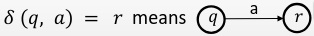
\includegraphics[width=0.3\linewidth]{Pictures/finite_auto_2.png}
    \end{figure}
    \item $q_0$ is the start state.
    \item $F$ is the set of accept states. 
\end{itemize}
\end{definition}

$\quad$\\[-1em]
\textbf{Example:}\\
Let's consider the following finite automaton.
\begin{figure}[H]
    \centering
    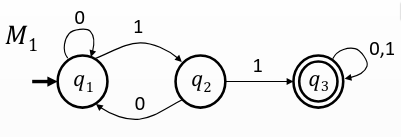
\includegraphics[width=0.4\linewidth]{Pictures/finite_auto_1.png}
\end{figure}
$\quad$\\[-2em]
Here, $M_1=(Q,\Sigma,\delta,q_1,F)$ is a finite automaton. For sake of example, here are the exact details of $M_1$.
\begin{itemize}
    \item $Q=\{q_1, q_2. q_3\}$
    \item $\Sigma=\{0, 1\}$
    \item $F=\{q_3\}$
\end{itemize}
It accepts a finite string as input. The output is either \textit{ACCEPT} or \textit{REJECT}.
The computation goes as follows:
\begin{enumerate}
    \item Begin at start state.
    \item Read input symbols.
    \item Follow corresponding transitions.
    \item \textit{ACCEPT} if we reach the accept state, otherwise \textit{REJECT}.
\end{enumerate}
For example: 01101 $\to$ \textit{ACCEPT}, while 00101 $\to$ \textit{REJECT}. Here, $M_1$ accepts all string in $A$ where $A=\{w|w\text{ contains substring }11\}$.
We say that \textbf{$A$ is the language of $M_1 \iff M_1$ recognizes $A \iff A=L(M_1)$}.

\subsection{Strings and languages}
A \textbf{string} is a finite sequence of symbols $w_1w_2\cdots w_n\in\Sigma$. A \textbf{language} is a set of string (finite or infinite).
The \textbf{empty string} $\epsilon$ is the string of length 0. The \textbf{empty language} $\emptyset$ is the set with no strings.
\begin{definition}[Accepting strings]
A finite automaton $M$ \textbf{accepts string} $w=w_1w_2\cdots w_n$ for each $w_i\in\Sigma$ 
if there exists a sequence of states $r_0,r_1,\dots,r_n\in Q$ where:
\begin{itemize}
    \item $r_0=q_0$
    \item $r_i=\delta(r_{i-1},w_i)$ for $1\leq i\leq n$
    \item $r_n\in F$
\end{itemize}
\end{definition}
\begin{definition}[Regular language]
We say a language is $\textbf{regular}$ if some finite automaton recognizes it.
\end{definition}
$\quad$\\[-1em]
\textbf{Example 1:}
\begin{figure}[H]
    \centering
    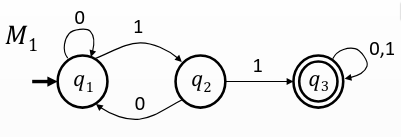
\includegraphics[width=0.4\linewidth]{Pictures/finite_auto_1.png}
\end{figure}
$\quad$\\[-1em]
$L=(M_1)=\{w|w\text{ contains substring }11\}=A$. Therefore, $A$ is regular.
\\\\
\textbf{Example 2:}\\
Let $B=\{w|w\text{ has an even number of 1s}\}$. In this case, $B$ is regular. (not shown)
\\\\
\textbf{Example 3:}\\
Let $C=\{w|w\text{ has equal number of 0s and 1s}\}$. In this case, $C$ is not regular. (provable)

\subsection{Regular expressions}
\begin{definition}[Regular operations]
Let $A,B$ be languages.
\begin{itemize}
    \item \textbf{Union:} $A\cup B=\{w|w\in A\text{ or }w\in B\}$.
    \item \textbf{Concatenation:} $A\circ B=\{xy|x\in A \text{ and }y\in B\}=AB$.
    \item \textbf{Star:} $A^{\star}=\{x_1\dots x_k|x_i\in A\text{ for }k\geq 0\}$. (Note: $\epsilon\in A^{\star}$)
\end{itemize}
\end{definition}
$\quad$\\[-1em]
Regular expressions are built from $\Sigma,\emptyset,\epsilon$ by using regular operations $\cup,\circ,\star$.
\\\\
\textbf{Example 1:}
\begin{itemize}
    \item $(0\cup 1)^{\star}=\Sigma^{\star}$ gives all strings over $\Sigma$.
    \item $\Sigma^{\star}1$ gives all strings that end with 1.
    \item $\Sigma^{\star}11\Sigma^{\star}$ gives all strings that contain $11=L(M_1)$.
\end{itemize}
\textbf{Example 2:}\\
Let $A=\{\text{good, bad}\}$ and $B=\{\text{boy, girl}\}$.
\begin{itemize}
    \item $A\cup B=\{\text{good, bad, boy, girl}\}$.
    \item $A\circ B=AB=\{\text{goodboy, goodgirl, badboy, badgirl}\}$.
    \item $A^{\star}=\{\epsilon, \text{good, bad, goodgood, goodbad, badgood, badbad, goodgoodgood, }\dots\}$
\end{itemize}

\end{document}